\chap{非磁性不純物効果を含む極低温フェルミ原子気体の強結合理論}\label{chap:formalism}

この章では、本論文で扱う理論の説明を行う。
\ref{sec:form:hami} 節では本論文で扱う非磁性不純物を含むフェルミ原子気体を記述するハミルトニアンを提示し、原子間相互作用の取り扱い方を \ref{sec:form:askfi} 節、不純物の取り扱い方を \ref{sec:form:imp} 節で説明する。
\ref{sec:form:bcsl} 節で、絶対零度における BCS-Legget 理論を不純物が存在する場合に拡張する。\ref{sec:form:tmat} 節では、超流動転移温度以上の超流動揺らぎの効果を取り入れた強結合理論を不純物が存在する場合に拡張する。

\s{モデルハミルトニアン}\label{sec:form:hami}
% \s{ハミルトニアン} \label{sec:form:hami}

次のハミルトニアンで表される、2 成分フェルミ原子気体を考える。
\beq
\hanaH &= \Hkin + \Hint + \Himp.\label{eq:form:ham:total}
\eeq
ここで、$\Hkin$ は自由フェルミ原子の運動エネルギー項、$\Hint$ はフェルミ間の接触型引力相互作用、そして $\Himp$ は非磁性不純物を表す。以下、これら各項について説明する。

先ず、運動エネルギー項 $\Hkin$ は第 2 量子化表示で次式で与えられる。
\beq
&\Hkin =  \sum_{\bp, \spin} \left( \ken_{\bp} - \cpt \right) c_{\bp \spin}^{\dag} c_{\bp \spin}. \label{eq:form:ham:hkin}
\eeq
ここで、$c_{\bp \spin}$ は運動量 $\bp$、(クーパー対形成に関与する 2 つの超微細構造状態を表す)擬スピン $\spin = \uar, \dar$ のフェルミ原子の消滅演算子を表す。$\ken_{\bp} = \bp^2 / (2m)$ はフェルミ原子の運動エネルギーで $m$ は原子の質量である。$\cpt$ は化学ポテンシャルである。


フェルミ原子間にはたらく引力相互作用を表す $\Hint$ は、
\beq
&\Hint = - \uint \sum_{\bp, \bpp, \bq}c_{\bp+\bqt,\uar}^{\dag} c_{-\bp+\bqt,\dar}^{\dag} c_{-\bpp + \bqt, \dar} c_{\bpp+\bqt, \uar}.\label{eq:form:ham:hint}
\eeq
ここでは接触型相互作用を考えているため、相互作用は逆向きの擬スピン間にのみはたらく。また $U$ は引力相互作用の強度を表す。ここでは $\Lisix$ や $\Kafor$ フェルミ原子気体を考え、$U$ はフェッシュバッハ共鳴により可変であるとする。

式 (\ref{eq:form:ham:total}) の右辺最終項は非磁性不純物散乱を表し、
\beq
&\Himp =  \sum_{i=1}^{\Nimp}\sum_{\bp, \bpp, \spin} e^{i(\bp-\bpp)\cdot \bri} \vimp c_{\bp\spin}^{\dag}c_{\bpp \spin},\label{eq:form:ham:himp}
\eeq
である。ここで、 $\vimp$ は不純物の散乱ポテンシャル、$\Nimp$ は不純物の数、$\bri$ は $i$ 番目の不純物の位置を表す。不純物散乱が擬スピン $\spin$ を変えず、さらに $\spin=\uar, \dar$  に対して同じ強度で散乱することから、非磁性不純物を表していることがわかる。

\ref{sec:form:bcsl} 節では、絶対零度の超流動状態を扱うが、その場合には 2 成分 Nambu 表示を用いるのが便利である。2 成分 Nambu 場、
\beq
\psip = \begin{pmatrix}c_{\bp, \uar}\\ c_{-\bp,\dar}^{\dag}\end{pmatrix},
\eeq
を用い、重要でない定数項を無視すると、式 (\ref{eq:form:ham:hkin}), (\ref{eq:form:ham:hint}), (\ref{eq:form:ham:himp}) の各項はぞれぞれ次のように書き表される:
\beq
&\hkin = \sum_{\bp} \psipd\  \left[ \ken_{\bp}-\cpt \right]\tau_3 \psip,\label{eq:form:ham:shkin}\\
&\hint = -\uint\sum_{\bq}\rho_+(\bq) \rho_-(-\bq) ,\label{eq:form:ham:shint}\\
&\himp = \sum_{i=1}^{\nimp} \sum_{\bp,\bpp} e^{i(\bp-\bpp) \cdot \bri} \psipd \vimp \tau_3 \vpsi_{\bp'}.\label{eq:form:ham:shimp}
\eeq
ここで、
\beq
\tau_1=\begin{pmatrix} 0 & 1 \\ 1 & 0 \end{pmatrix},\ \tau_2=\begin{pmatrix} 0 & -i \\ i & 0 \end{pmatrix}, \ \tau_1=\begin{pmatrix} 1 & 0 \\ 0 & -1 \end{pmatrix},\notag
\eeq
はパウリ行列である。式 (\ref{eq:form:ham:shint}) において、$\rho_s(\bq)$ は一般化された密度演算子であり、次式で与えられる。
\beq
\rho_{\pm} = \sum_{\bp} \varPsi^{\dag}_{\bp} \tau_{\pm} \varPsi_{\bp-\bq}.
\eeq
ここで、
\beq
\tau_+ = \frac{1}{2} \left[ \tau_1 + i \tau_2 \right] = \begin{pmatrix}0& 1 \\ 0& 0\end{pmatrix},\\
\tau_- = \frac{1}{2} \left[ \tau_1 - i \tau_2 \right] = \begin{pmatrix}0& 0 \\ 1& 0\end{pmatrix},
\eeq
を用いた。

\s{フェルミ原子間相互作用 $\Uint$ に対する $s$ 波散乱長 $\as$}\label{sec:form:askfi}


冷却フェルミ原子気体の分野では原子間相互作用の強さは、通常、裸の相互作用 $U$ ではなく、$s$ 波散乱長 $\as$ として測定されるので、理論を構築する際も相互作用強度を $\as$ で与えられるように定式化しておくと、実際と比較する際都合が良い。また、前述したようにフェッシュバッハ共鳴に因る相互作用にはフォノン媒介型相互作用におけるデバイ周波数のような物理的なカットオフがない為、接触型相互作用に起因する紫外発散を除く必要があるが、後述するようにこれをくりこみ処理により散乱長 $\as$ に吸収させることができる。

式 (\ref{eq:form:ham:total}) のハミルトニアンの相互作用 $\Hint$ 中にある裸の相互作用 $U$ と $s$ 波散乱長$ \as$ の関係は次式で与えられる \cite{ohashi2005}。
\beq
\frac{ 4 \pi \as}{m} =  \frac{-\uint}{1 - \uint \sum_{p}^{\omega_c} \frac{1}{2 \ken_p}}.\label{eq:form:ham:askf}
\eeq
ここで $\omega_c$ は形式的に導入したカットオフエネルギーである。相互作用を $\as$ を用いて表すと相図 \ref{fig:bcsbecsouzu}にあるように $\askfi \ltsim -1$ が弱結合 BCS 領域($\tc$ 以下は平均場 BCS 状態に近い)、$\askfi \gtsim +1$ が強結合 BEC 領域($\tc$ 以上でも強い引力相互作用により 2 体束縛状態としての分子ボソンが形成される)となる。$-1 \ltsim \askfi \ltsim 1$ の領域はユニタリ領域、特に $\askfi \to 0\  (\as\to \pm\infty)$ は、ユニタリ極限と呼ばれる。ユニタリ領域は、フェルミ対の形成と解離の繰り返しで特徴付けられる超流動ゆらぎが顕著な領域である。

\s{有限濃度の不純物に対する分布平均と自己無撞着 $T$ 行列近似}\label{sec:form:imp}

式 (\ref{eq:form:ham:himp}) で記述される有限濃度の不純物は特定の不純物配置 $\{\bri\}$ に依存しており系の並進対称性が失われている。特定の不純物配置 $\{\bri\}$ に依存しない結果を得るために、ここでは様々な不純物の分布に関する平均をとる(その結果、理論としては並進対称性が回復する)。不純物の分布平均の取り方には様々な方法があるが、ここでは金属電子系で用いられてきた、自己エネルギーに対する不純物の位置平均を採用する。すなわち与えられた自己エネルギー $\sig^{\imp}_{\bp, \bpp}(i \omn, \bm{R}_1, \bm{R}_2, \dots, \bm{R}_{\nimp})$ に対し(ここで $\omn = \pi T(2 n + 1)$、$n=0, \pm1, \dots$ はフェルミオン松原周波数)、不純物の分布平均をとった自己エネルギー $\sigimppom$ を次式で与える。
\beq
\sigimppom \delta_{\bp,\bpp} = \frac{1}{V^{\nimp}}\int \diff \bm{R}_1 \cdots \diff \bm{R}_{\nimp}  \sig^{\imp}_{\bp, \bpp}(i \omn, \bm{R}_1, \bm{R}_2, \dots, \bm{R}_{\nimp}).
\eeq
ここでは、体積 $V$ を明示した。この方法は、金属超伝導の不純物効果の研究でも用いられている \cite{abrikosov1961,shiba1968, shiba1973}。この操作により並進対称性が回復するので、自己エネルギーは運動量について対角的になる。左辺のクロネッカーデルタ $\delta_{\bp, \bpp}$ はそれを反映したものである。

\begin{figure}[t]
\begin{center}
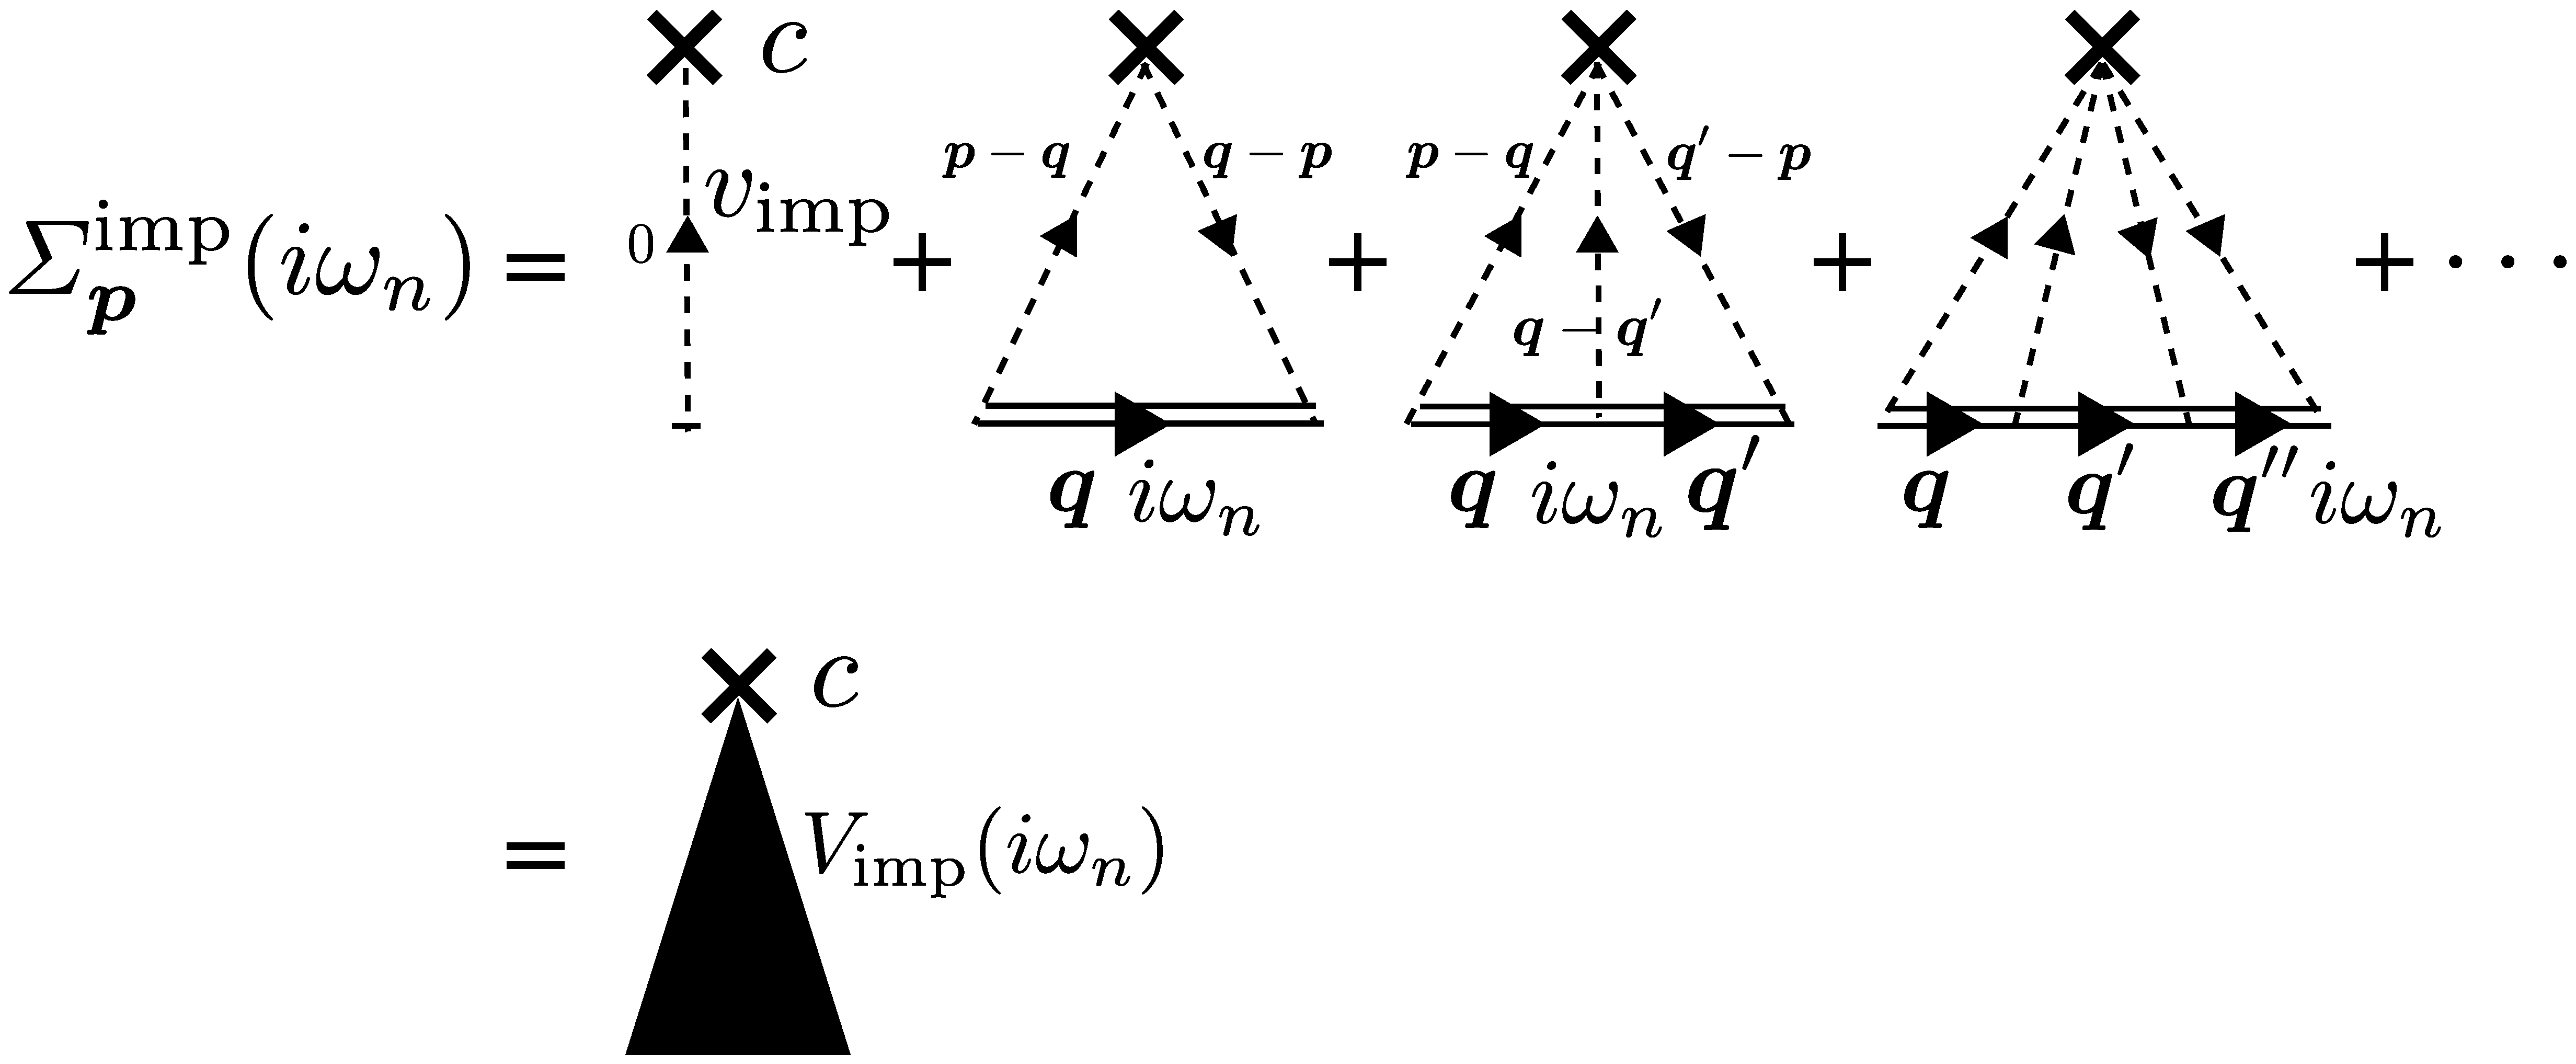
\includegraphics[width=120mm]{eps/sig-impimp.eps}
\end{center}
\caption{非磁性不純物散乱に対する自己無撞着 $T$ 行列近似を表すファインマンダイアグラム。図中、破線は不純物散乱ポテンシャル $\vimp$、二重線は 1 粒子温度グリーン関数 $\gimppom$、$\times$ 印は不純物濃度 $c$ を表す。この近似は、一つの不純物による任意回の不純物散乱を含み、内線も不純物散乱の自己エネルギーを含むグリーン関数 $\gimppom$ が用いられている。これら多重散乱をまとめたものが有効不純物散乱ポテンシャル $\vvtxn$ である。}
\label{fig:form:ham:sigimp}
\end{figure}


不純物散乱 $\Himp$ に対し自己無撞着 $T$ 行列近似を採用する。この近似は図 \ref{fig:form:ham:sigimp} のダイアグラムで表され、分布平均をとった後の系のグリーン関数を $\gimppom$ とすると自己エネルギーは、
\beq
\sigimppom &= \con \vimp \frac{1}{1 - \vimp \sum_{\bq} \gimp_{\bq}(i\omn)}\notag\\
& \equiv \con \vvtxn,\label{eq:form:ham:sctma}
\eeq 
となる。ここで、 $c=\nimp/V$($V$ は体積)は不純物濃度である。式 (\ref{eq:form:ham:sctma}) の $\vvtxn$ は不純物の多重散乱を含む有効不純物散乱ポテンシャルを表し、図 \ref{fig:form:ham:sigimp} の二行目の黒三角形のダイアグラムに対応する。本論文では用いないが、式 (\ref{eq:form:ham:sctma}) 中のグリーン関数 $\gimppom$ を無摂動のグリーン関数、
\beq
\gzrpom = \frac{1}{i \omn - \left[ \varepsilon_{\bp}- \cpt\right]},
\eeq
で置き換えたものは $T$ 行列近似と呼ばれる。

不純物濃度は体積濃度、
\beq
c = \frac{\nimp}{V},\label{eq:form:ham:cvolume}
\eeq
として定義されているので、ダイアグラム法を用いる際には図 \ref{fig:form:ham:sigimp} 中の $\times$ 印に $c$ を割り当てれば良い。本論文では $V=1$ としているため、式 (\ref{eq:form:ham:cvolume}) の $c$ は無次元量であるが、計算結果に対し議論をする際にはフェルミ原子数 $N$ で規格化した濃度、
\beq
\overline{c}=\frac{\nimp}{N} = \frac{4}{3} \frac{c}{\fdos \eqf},\label{eq:form:ham:overlinec}
\eeq
を用いると便利である。ここで $\eqf = \kf^2/(2m)$ はフェルミエネルギーであり、
\beq
\fdos = \frac{mk_{\text{F}}}{2\pi^2},
\eeq
は自由フェルミ気体のフェルミ面における 1 粒子状態密度である。

今考えているモデルでは、不純物散乱も式 (\ref{eq:form:ham:himp}) から分かるように接触型を仮定しているので、式 (\ref{eq:form:ham:sctma}) は紫外発散を含む。そこでこれを除去するために不純物散乱ポテンシャル $\vimp$ に対する $s$ 波散乱長 $\bs$ を導入し、引力相互作用の時と同様、紫外発散を $\bs$ にくりこむ。散乱長 $\bs$ は“裸”の不純物散乱ポテンシャル $\vimp$ と次式で関係付けられる:
 \beq
 \frac{2 \pi \bs}{m} = \frac{\vimp}{1-\vimp\sum_p^{\omega_c'} \frac{1}{ \ken_{\bp}}}.\label{eq:form:ham:bskf}
\eeq
ここで、$\omega_c'$ は形式的に導入したエネルギーカットオフである。散乱長 $\bs$ を用いると式 (\ref{eq:form:ham:sctma}) の自己エネルギーは、
\beq
\sigimppom = c\frac{1}{\frac{m}{2\pi \bs} - \sum_{\bq} \left[ \gimp_{\bq}(i\omn) + \frac{1}{ \ken_{\bq}} \right]},\label{eq:form:ham:sctmabs}
\eeq
となり、式 (\ref{eq:form:ham:sctma}) の分母の運動量和が持っていた紫外発散は $\bs$ に吸収されて式 (\ref{eq:form:ham:sctmabs}) からは除かれる(式 (\ref{eq:form:ham:sctmabs})の分母の $\bq$ の和は紫外発散しないことに注意)。

式 (\ref{eq:form:ham:sctma}) において、分母を陽に現れている $\vimp$ に対し 2 次まで展開した上で、 1 次の定数項 $c \vimp$ は定数シフトとして $\cpt$ に吸収させて無視したもの、
\beq
\varSigma^{\text{Born}}_{\text{imp}} ( i \omn) &= c \vimp^2 \sum_{\bq} \gimp_{\bq}(i\omn) = c \left[\frac{1}{\frac{m}{2 \pi \bs} - \sum_{\bq}^{\omega_c}\frac{1}{\ken_{\bq}}}\right]^2 \sum_{\bq} \gimp_{\bq}(i\omn) ,\label{eq:form:ham:scborn}
\eeq 
は自己無撞着ボルン近似と呼ばれ、化学ポテンシャルシフト以上の効果を与える最低次のみを取り出した近似として金属超伝導体に対する不純物効果の研究でよく用いられている。しかし、フェルミ原子気体の場合には、式 (\ref{eq:form:ham:scborn}) を用いると $\bs$ を導入しても物理的なカットオフが存在しないため、非物理的なカットオフに顕わに依存した表式となってしまう。このため、本研究では自己無撞着ボルン近似は用いない。

最後に、不純物散乱に対する自己無撞着 $T$ 行列近似を超伝導状態で考える際に便利な Nambu 表示での表式について説明する。式 (\ref{eq:form:ham:shkin})-(\ref{eq:form:ham:shimp}) のように Nambu 表示すると、不純物散乱には $\tau_3$ が掛かる。結果、Nambu 表示の下での自己エネルギー $\bsigimppom$ は、
\beq
\bsigimppom &= \con \bvvtxn=\con \frac{1}{\frac{m}{2\pi \bs}\tau_3 - \sum_{\bq} \left[ \bgimp_{\bq}(i\omn) + \frac{\tau_3}{ \ken_{\bq}} \right]},\label{eq:form:ham:abcslimp}
\eeq 
となる。ここで、
\beq
\bgimp_{\bp}(i\omn) = \frac{1}{i \omn - \left[\ken_{\bp} - \cpt\right]\tau_3 - \bsigimppom},
\eeq
は2 成分 Nambu 場を用いた $2 \times 2$ 行列の 1 粒子温度グリーン関数である。
%%%%%%%%%%%%%%%%%%%%%%%%%%%%%%%%%%%%%%%%%%%%%%%%%%%%%%%%%%%%

\s{BCS-Leggett 理論の非磁性不純物効果を含む場合への拡張}\label{sec:form:bcsl}
% \s{�񎥐��s�������ʂ��܂� BCS-Legett ���_}\label{sec:form:bcsl}

�����ł́A$T=0$ �̒��������ɂ����钴���������p�����[�^ $\del$ �Ɖ��w�|�e���V���� $\cpt$ ��񎥐��s���������݂���ꍇ�ɁABCS-BEC �N���X�I�[�o�[�S��Ō��肷�邽�߂̗��_�I�g�g�݂��������B�{�����ł� BCS-Leggett ���_��p���邪�A���ۂɂ́A�L�����x�̏����`���Œ莮�����s���A���x���\���������Ƃ�i$T=0.01\eqf$�j���ƂŐ�Η�x�̌v�Z�Ƃ���i����� $\del \gg 0.01\eqf$ �ł���Ηǂ��ߎ��ł���j�B�܂��ANambu �\���ł̃n�~���g�j�A���ł��鎮 (\ref{eq:form:ham:shkin}), (\ref{eq:form:ham:shint}), (\ref{eq:form:ham:shimp}) ��p����B

\begin{figure}[t]
\begin{center}
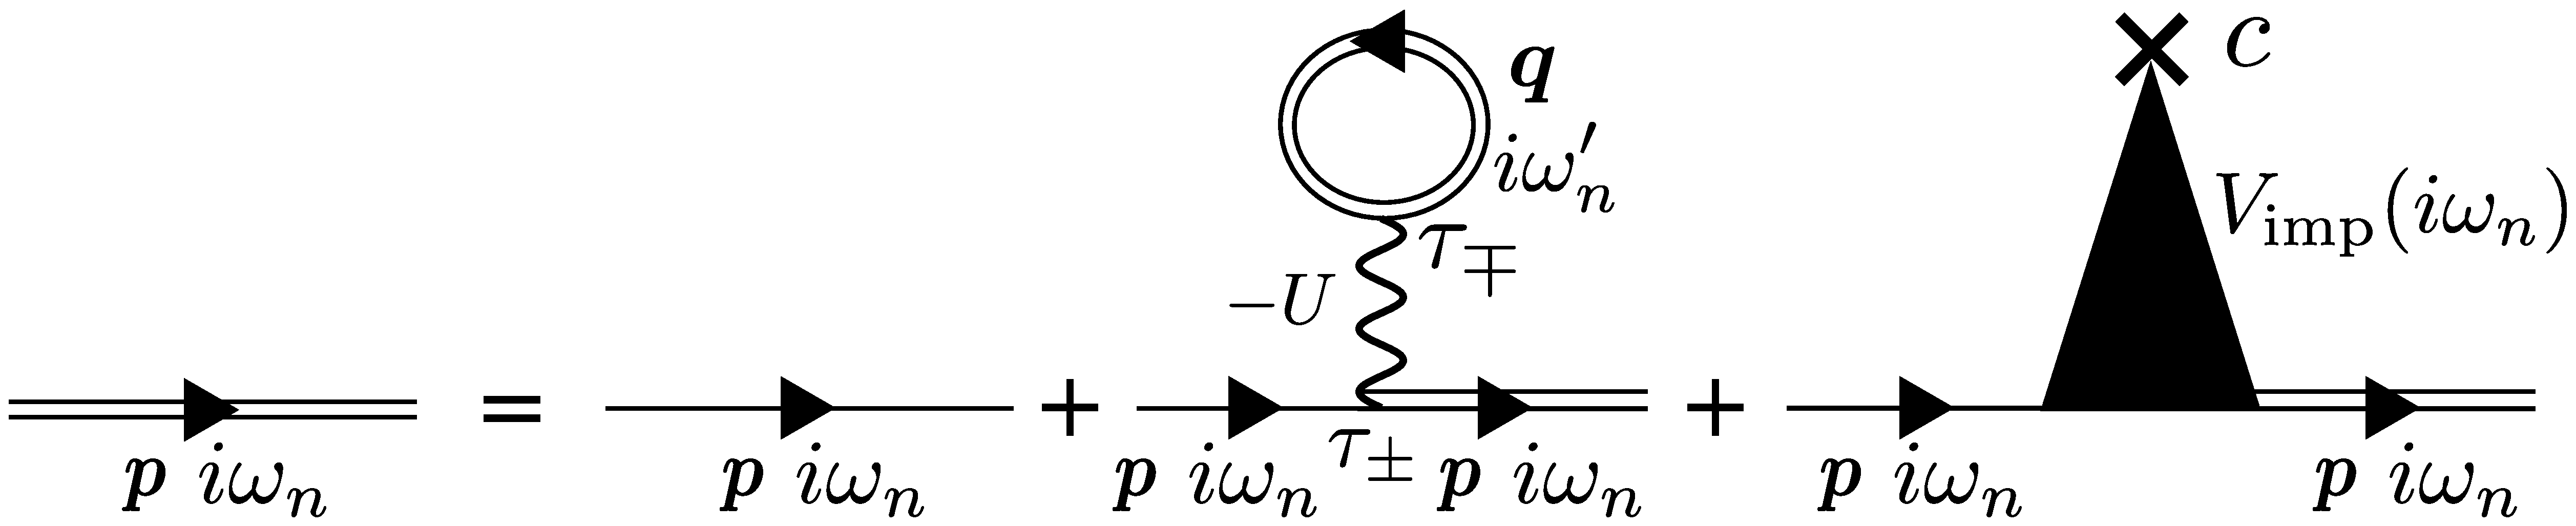
\includegraphics[width=125mm]{eps/dyson-vimp.eps}
\end{center}
\caption{�񎥐��s�������ʂ��܂� BCS-Leggett ���_�B�����͖��ۓ��̃O���[���֐� $\gzrpom$�A��d���͑S�n�̃O���[���֐� $\bgimppom$�A�g���̓t�F�b�V���o�b�n���‚ɂ��t�F���~�I���ԑ��ݍ�p $-U$�A$\times$ ��͕s�����Z�x $c$�A���O�p�`�͕s�����ɂ��L���U�����x $\vvtxn$ ��\���B}
\label{fig:form:mnf:sigimp}
\end{figure}

 1 ���q���x�O���[���֐��͎��̃_�C�\���������𖞂����B
 \beq
\left[ \bgimppom \right]^{-1} = \bgzrpom^{-1} - \bsigpom.\label{eq:form:mnf:dyson0}
\eeq
������ $\bgzrpom$ �͎��R�t�F���~�C�̂ɂ����� Nambu �\���ł̃O���[���֐��ł���A�����ŗ^������B
\beq
\bgzrpom = \frac{1}{i \omn - \left[ \ken_{\bp}- \cpt\right] \tau_3}.
\eeq

BCS-Leggett ���_�̘g�g�݂ł͎��ȃG�l���M�[�͐} \ref{fig:form:mnf:sigimp} �̉E�� 1 ���ڂ� 2 ���ڂ̘a�ŗ^�����A�񎥐��s�������܂ޏꍇ�͂���ɐ} \ref{fig:form:mnf:sigimp}  �̍ŏI���������B

���A���ȃG�l���M�[�𑊌ݍ�p�̊�^ $\bsigintpom$ �ƕs�����U�� $\bsigimppom$ �ɕ����A
\beq
\bsigpom = \bsigintpom + \bsigimppom.\label{eq:form:mnf:sig}
\eeq
�Ƃ����ƁA���q�ԑ��ݍ�p�ɂ�镔���́A�} \ref{fig:form:mnf:sigimp} �̉E�� 2 ���ڕ������瓾���A
\beq
\bsigintpom = - \frac{U}{\beta} \sum_{\omn'} \sum_{\bpp}\left[\tau_-\Tr \left[ \tau_+ \bgimppomp  e^{i\omn'\delta}\right]+ \tau_+ \Tr \left[ \tau_- \bgimppomp  e^{i\omn'\delta}\right] \right],\label{eq:form:mnf:intpom}
\eeq
�ƂȂ�B�����������p�����[�^ $\del$ �� Nambu �\���̃O���[���֐���p���A���̂悤�ɏ������Ƃ��ł���B
\beq
\varDelta = U \sum_{\bpp} \braket{c_{-\bpp\dar}c_{\bpp\uar}} = \frac{U}{\beta} \sum_{\omn'}\sum_{\bpp} \Tr \left[ \tau_- \bgimppomp e^{i\omn'\delta} \right].\label{eq:form:mnf:gapeq0}
\eeq
��ʐ����������ƂȂ��A$\del$ �����ƂȂ�悤�Ɉʑ���I�ԂƁA�� (\ref{eq:form:mnf:intpom}) �̎��ȃG�l���M�[�͎��̂悤�ɂ܂Ƃ܂�B
\beq
\bsigintpom =  - \del \tau_1.\label{eq:form:mnf:delsig}
\eeq
�����s�����U�����Ȃ���΁A�� (\ref{eq:form:mnf:delsig}) ���� (\ref{eq:form:mnf:dyson0}) �ɑ�����ē�����O���[���֐��A
\beq
\bgpom = \frac{1}{i\omn - \left[ \ken_{\bp} - \cpt \right]\tau_3 + \del \tau_1}
\eeq
�́ANambu �\���̉��ł́i�s�������܂܂Ȃ��ꍇ�́jBCS �n�~���g�j�A���A
\beq
\hanah_{\text{BCS}} = \sum_{\bp}\varPsi_{\bp}^{\dag} \left[ \left[\ken_{\bp} - \cpt\right] \tau_3 - \del \tau_1 \vphantom{\frac{1}{2}}\right] \varPsi_{\bp},
\eeq
���瓾���� 1 ���q���x�O���[���֐��Ɉ�v����B

�񎥐��s�������ʂ�\�����ȃG�l���M�[ $\bsigimppom$ �͎� (\ref{eq:form:ham:abcslimp}) �ŗ^�����鎩�Ȗ����� $T$ �s��ߎ��̕\����p����B�������ē���ꂽ�񎥐��s���������݂���ꍇ�Ɋg�����ꂽ BCS-Leggett ���_�ɂ����� 1 ���q�O���[���֐��́A
\beq
\bgimppom &= \frac{1}{i \omn - \left[ \ken_{\bp}- \cpt \right]\tau_3 + \del \tau_1 - \bsigimppom}\notag\\
&\equiv \frac{1}{i \tomn - \left[ \ken_{\bp} - \tcptn\right]\tau_3 + \tdeln \tau_1}.\label{eq:form:mnf:gimpopmpom}
\eeq
�ƂȂ�B�����ŁA�� (\ref{eq:form:mnf:gimpopmpom}) 2 �s�ڂ͕s�����U�����ʂ�\�����ȃG�l���M�[ $\bsigimppom$ �̌��ʂ��A�������g���i$\omn \to \tomn$�j�A�����������p�����[�^�i$\del \to \tdeln$�j�A����щ��w�|�e���V�����i$\cpt \to \tcptn$�j�ɂ��肱�񂾕\���ł���B�� (\ref{eq:form:ham:abcslimp}) �̕���ɂ‚��āA
\beq
\sum_{\bp} \bgimppom = \sum_{\bp} \frac{1}{i\tomn - (\ken_{\bp} - \tcptn) \tau_3 + \tdeln \tau_1} = -\sum_{\bp}\frac{i\tomn - \tdeln \tau_1 + (\ken_{\bp} - \tcptn) \tau_3}{\tomn^2 + \tdeln^2 + (\ken_{\bp}-\tcptn)^2},\label{eq:form:mnf:sumg}
\eeq
�Ə�����邱�Ƃɒ��ӂ���ƁA���̕\������ (\ref{eq:form:ham:abcslimp}) �ɑ��������ŁA�� (\ref{eq:form:mnf:gimpopmpom}) 1 �s�ڂɑ������B���̎� (\ref{eq:form:mnf:gimpopmpom}) �� 1 �s�ڂ� 2 �s�ڂ��r���Ċe�p�E���s��̌W�����m�𓙂����ƒu�����ƂŁA���� 3 �‚̎��Ȗ������������𓾂�B
\beq
\tomn &= \omn + c \frac{\frac{\tomn}{\sqrt{\tomn^2 + \tdeln^2}} \sum_{\bp} \frac{\sqrt{\tomn^2+\tdeln^2}}{\tomn^2+\tdeln^2 + (\ken_{\bp}-\tcptn)^2}}{\left[\sum_{\bp} \frac{\sqrt{\tomn^2+\tdeln^2}}{\tomn^2+\tdeln^2 + (\ken_{\bp}-\tcptn)^2}\right]^2 + \left[\frac{m}{2\pi \bs} + \sum_{\bp} \left[\frac{\ken_{\bp}-\tcptn}{\tomn^2+\tdeln^2 + (\ken_{\bp}-\tcptn)^2}- \frac{1}{\ken_{\bp}} \right]\right]^2},\label{eq:form:mnf:tomn}\\
\tdeln &=\del + c \frac{\frac{\tdeln}{\sqrt{\tomn^2 + \tdeln^2}} \sum_{\bp} \frac{\sqrt{\tomn^2+\tdeln^2}}{\tomn^2+\tdeln^2 + (\ken_{\bp}-\tcptn)^2}}{\left[\sum_{\bp} \frac{\sqrt{\tomn^2+\tdeln^2}}{\tomn^2+\tdeln^2 + (\ken_{\bp}-\tcptn)^2}\right]^2 + \left[\frac{m}{2\pi \bs} + \sum_{\bp} \left[\frac{\ken_{\bp}-\tcptn}{\tomn^2+\tdeln^2 + (\ken_{\bp}-\tcptn)^2}- \frac{1}{\ken_{\bp}} \right]\right]^2},\label{eq:form:mnf:tdeln}\\
\tcptn &=\cpt - c \frac{\frac{m}{2\pi \bs} + \sum_{\bp} \left[\frac{\ken_{\bp}-\tcptn}{\tomn^2+\tdeln^2 + (\ken_{\bp}-\tcptn)^2}- \frac{1}{\ken_p} \right]}{\left[\sum_{\bp} \frac{\sqrt{\tomn^2+\tdeln^2}}{\tomn^2+\tdeln^2 + (\ken_{\bp}-\tcptn)^2}\right]^2 + \left[\frac{m}{2\pi \bs} + \sum_{\bp} \left[\frac{\ken_{\bp}-\tcptn}{\tomn^2+\tdeln^2 + (\ken_{\bp}-\tcptn)^2}- \frac{1}{\ken_{\bp}} \right]\right]^2}.\label{eq:form:mnf:tcptn}
\eeq
�� (\ref{eq:form:mnf:tomn}), (\ref{eq:form:mnf:tdeln}), (\ref{eq:form:mnf:tcptn}) �����Ȗ������ɉ����A�i$\tomn, \tdeln, \tcptn$�j�����肷�邱�ƂŁA�s�������ʂ��܂ތn�̃O���[���֐������܂�B

�� (\ref{eq:form:mnf:tomn}) �̗��ӂ� $\omn$ �Ŋ��������̂Ǝ� (\ref{eq:form:mnf:tdeln}) �̗��ӂ� $\del$ �Ŋ��������͓̂������B
\beq
\frac{\tomn}{\omn} = \frac{\tdeln}{\del}.\label{eq:form:mnf:nonmag}
\eeq
���̓�����p����ƁA�������`���ł悭�p������g���q-�z�[���Ώ̐��h�����肷�邱�ƂƁA1 ���q��Ԗ��x�̃G�l���M�[�ˑ����𖳎����邱�ƂŁA�A���_�[�\���̒藝���������邱�Ƃ��������Ƃ��ł���i�t�^ \ref{sec:append:anderson} �Q�Ɓj�B

BCS-Leggett ���_�ł́A$T=0$ �ɂ����钴���������p�����[�^~$\del$~�Ɖ��w�|�e���V����~$\cpt$~�́A�M���b�v������ (\ref{eq:form:mnf:gapeq0}) �ƁA���q���������A
\beq
N &= \sum_{\bp,\spin} \braket{c^{\dag}_{\bp\spin}c_{\bp\spin}} = \sum_{\bp} \left[1+\braket{c^{\dag}_{\bp\uar}c_{\bp\uar}}-\braket{c_{\bp\dar}c^{\dag}_{\bp\dar}}\right]\notag\\
& =  \sum_{\bp} \left[ 1 + \frac{1}{\beta} \sumn \Tr\left[ \tau_3 \bgimppom e^{i\omn \delta}\right] \right], \label{eq:form:mnf:numeq0}
\eeq
���猈�肳���B������ 2 �����A�� (\ref{eq:form:mnf:tomn})-(\ref{eq:form:mnf:tcptn}) �Ō��܂�J�荞�܂ꂽ�ϐ��i$\tomn, \tdeln, \tcptn$�j��p���ď��������ƁA�M���b�v������ (\ref{eq:form:mnf:gapeq0}) �Ɨ��q�������� (\ref{eq:form:mnf:numeq0}) �͂��ꂼ��A
\beq
&\frac{m}{4 \pi \as} + \sum_{\bp}\left[ \frac{1}{\beta}\sumn \frac{ \tdeln}{\del} \frac{1}{\tomn^2+\tdeln^2 + (\ken_{\bp}-\tcptn)^2} - \frac{1}{2 \ken_{\bp}}\right] = 0, \label{eq:form:mnf:gapeq}\\
&N = \sum_{\bp} \left[ 1 - \frac{2}{\beta}\sum_n \frac{ \ken_{\bp} - \tcptn}{\tomn^2+\tdeln^2+(\ken_{\bp}-\tcptn)^2} \right], \label{eq:form:mnf:numeq}
\eeq
�ƂȂ�B����� 2 �‚̕������ƌJ�荞�܂ꂽ�� �i$\tomn, \tdeln, \tcptn$�j�ɑ΂�������� (\ref{eq:form:mnf:tomn})-(\ref{eq:form:mnf:tcptn}) ��A�����ĉ������Ƃŕs�������܂ޒ�������Ԃ� BCS-BEC �N���X�I�[�o�[�̈�ɂ����� $\del$ �� $\cpt$ �����肳���B�{�����ł͂���𐔒l�I�ɍs���B

�񎥐��s�������܂܂Ȃ��N���[���Ȍn�̏ꍇ�́i$\tomn, \tdeln, \tcptn$�j$\to$ �i$\omn, \del, \cpt$�j�Ƃ��邱�ƂŒʏ�� BCS-Leggett ���_���Č������B�t�^ \ref{sec:append:pure:bcsl} �Ɍ��ʂ��܂Ƃ߂Ă���B



\s{非磁性不純物を含む有限温度のフェルミ原子気体の相互作用に対する $T$ 行列理論}\label{sec:form:tmat}
% \s{有限温度における非磁性不純物効果}\label{sec:form:tmat}

\begin{figure}[t]
\begin{center}
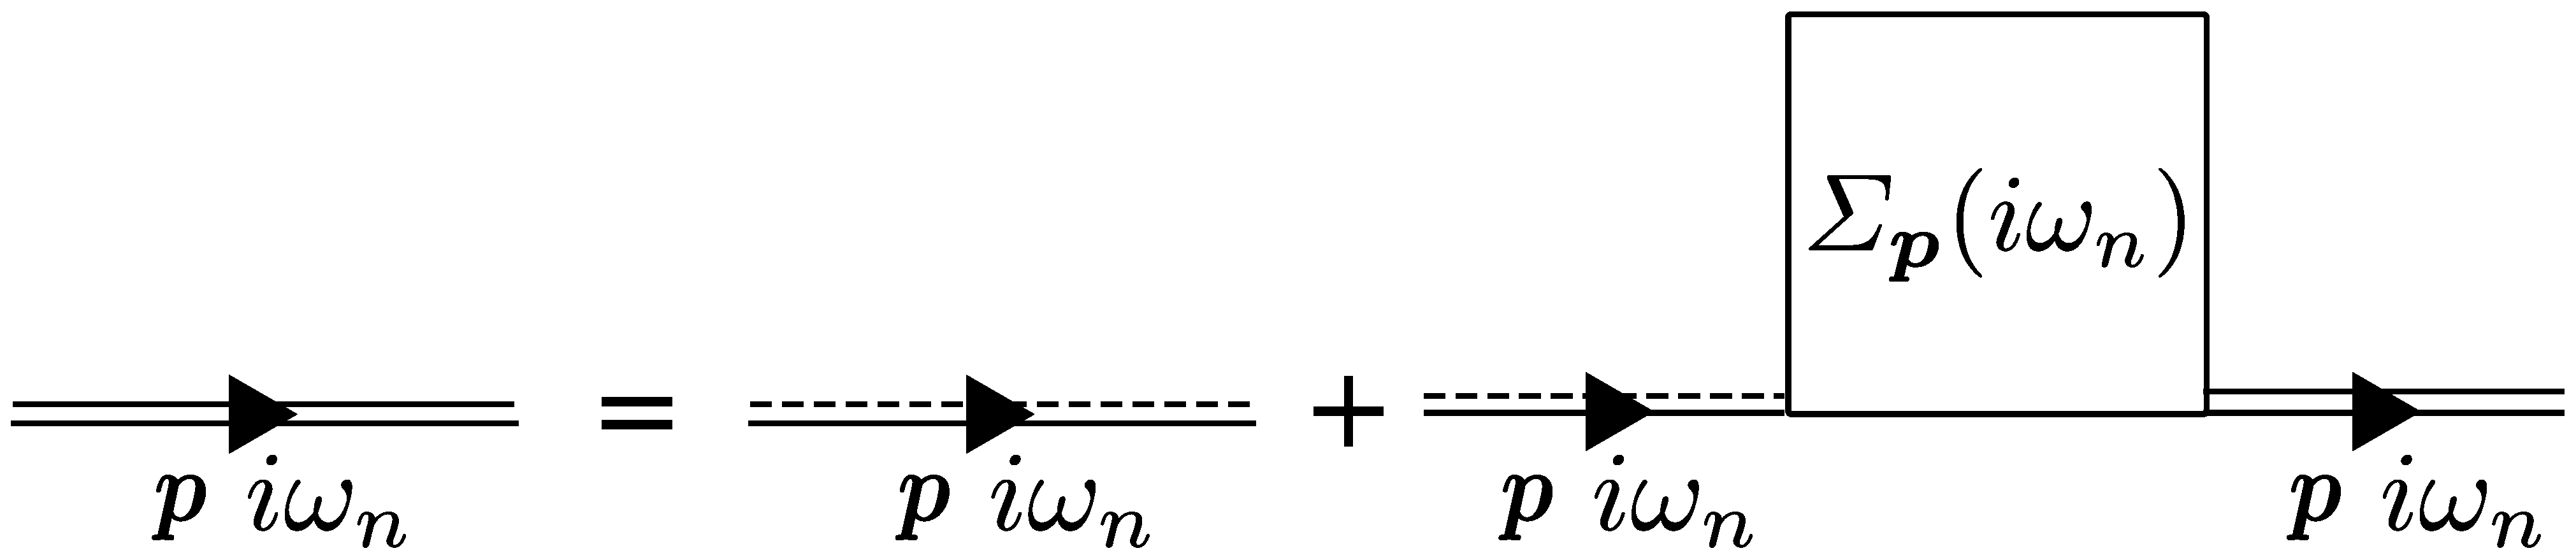
\includegraphics[height=20mm]{eps/dyson-tma-imp.eps}
\end{center}
\caption{原子間相互作用の効果を含む 1 粒子温度グリーン関数 $\gpom$ のダイソン方程式。二重実線は $\gpom$、破線と実線による二重線は不純物グリーン関数 $\gimppom$、$\sigpom$ は引力相互作用の効果を表す自己エネルギーである。}
\label{fig:form:tma:greenall}
\end{figure}


\begin{figure}[t]
\centering
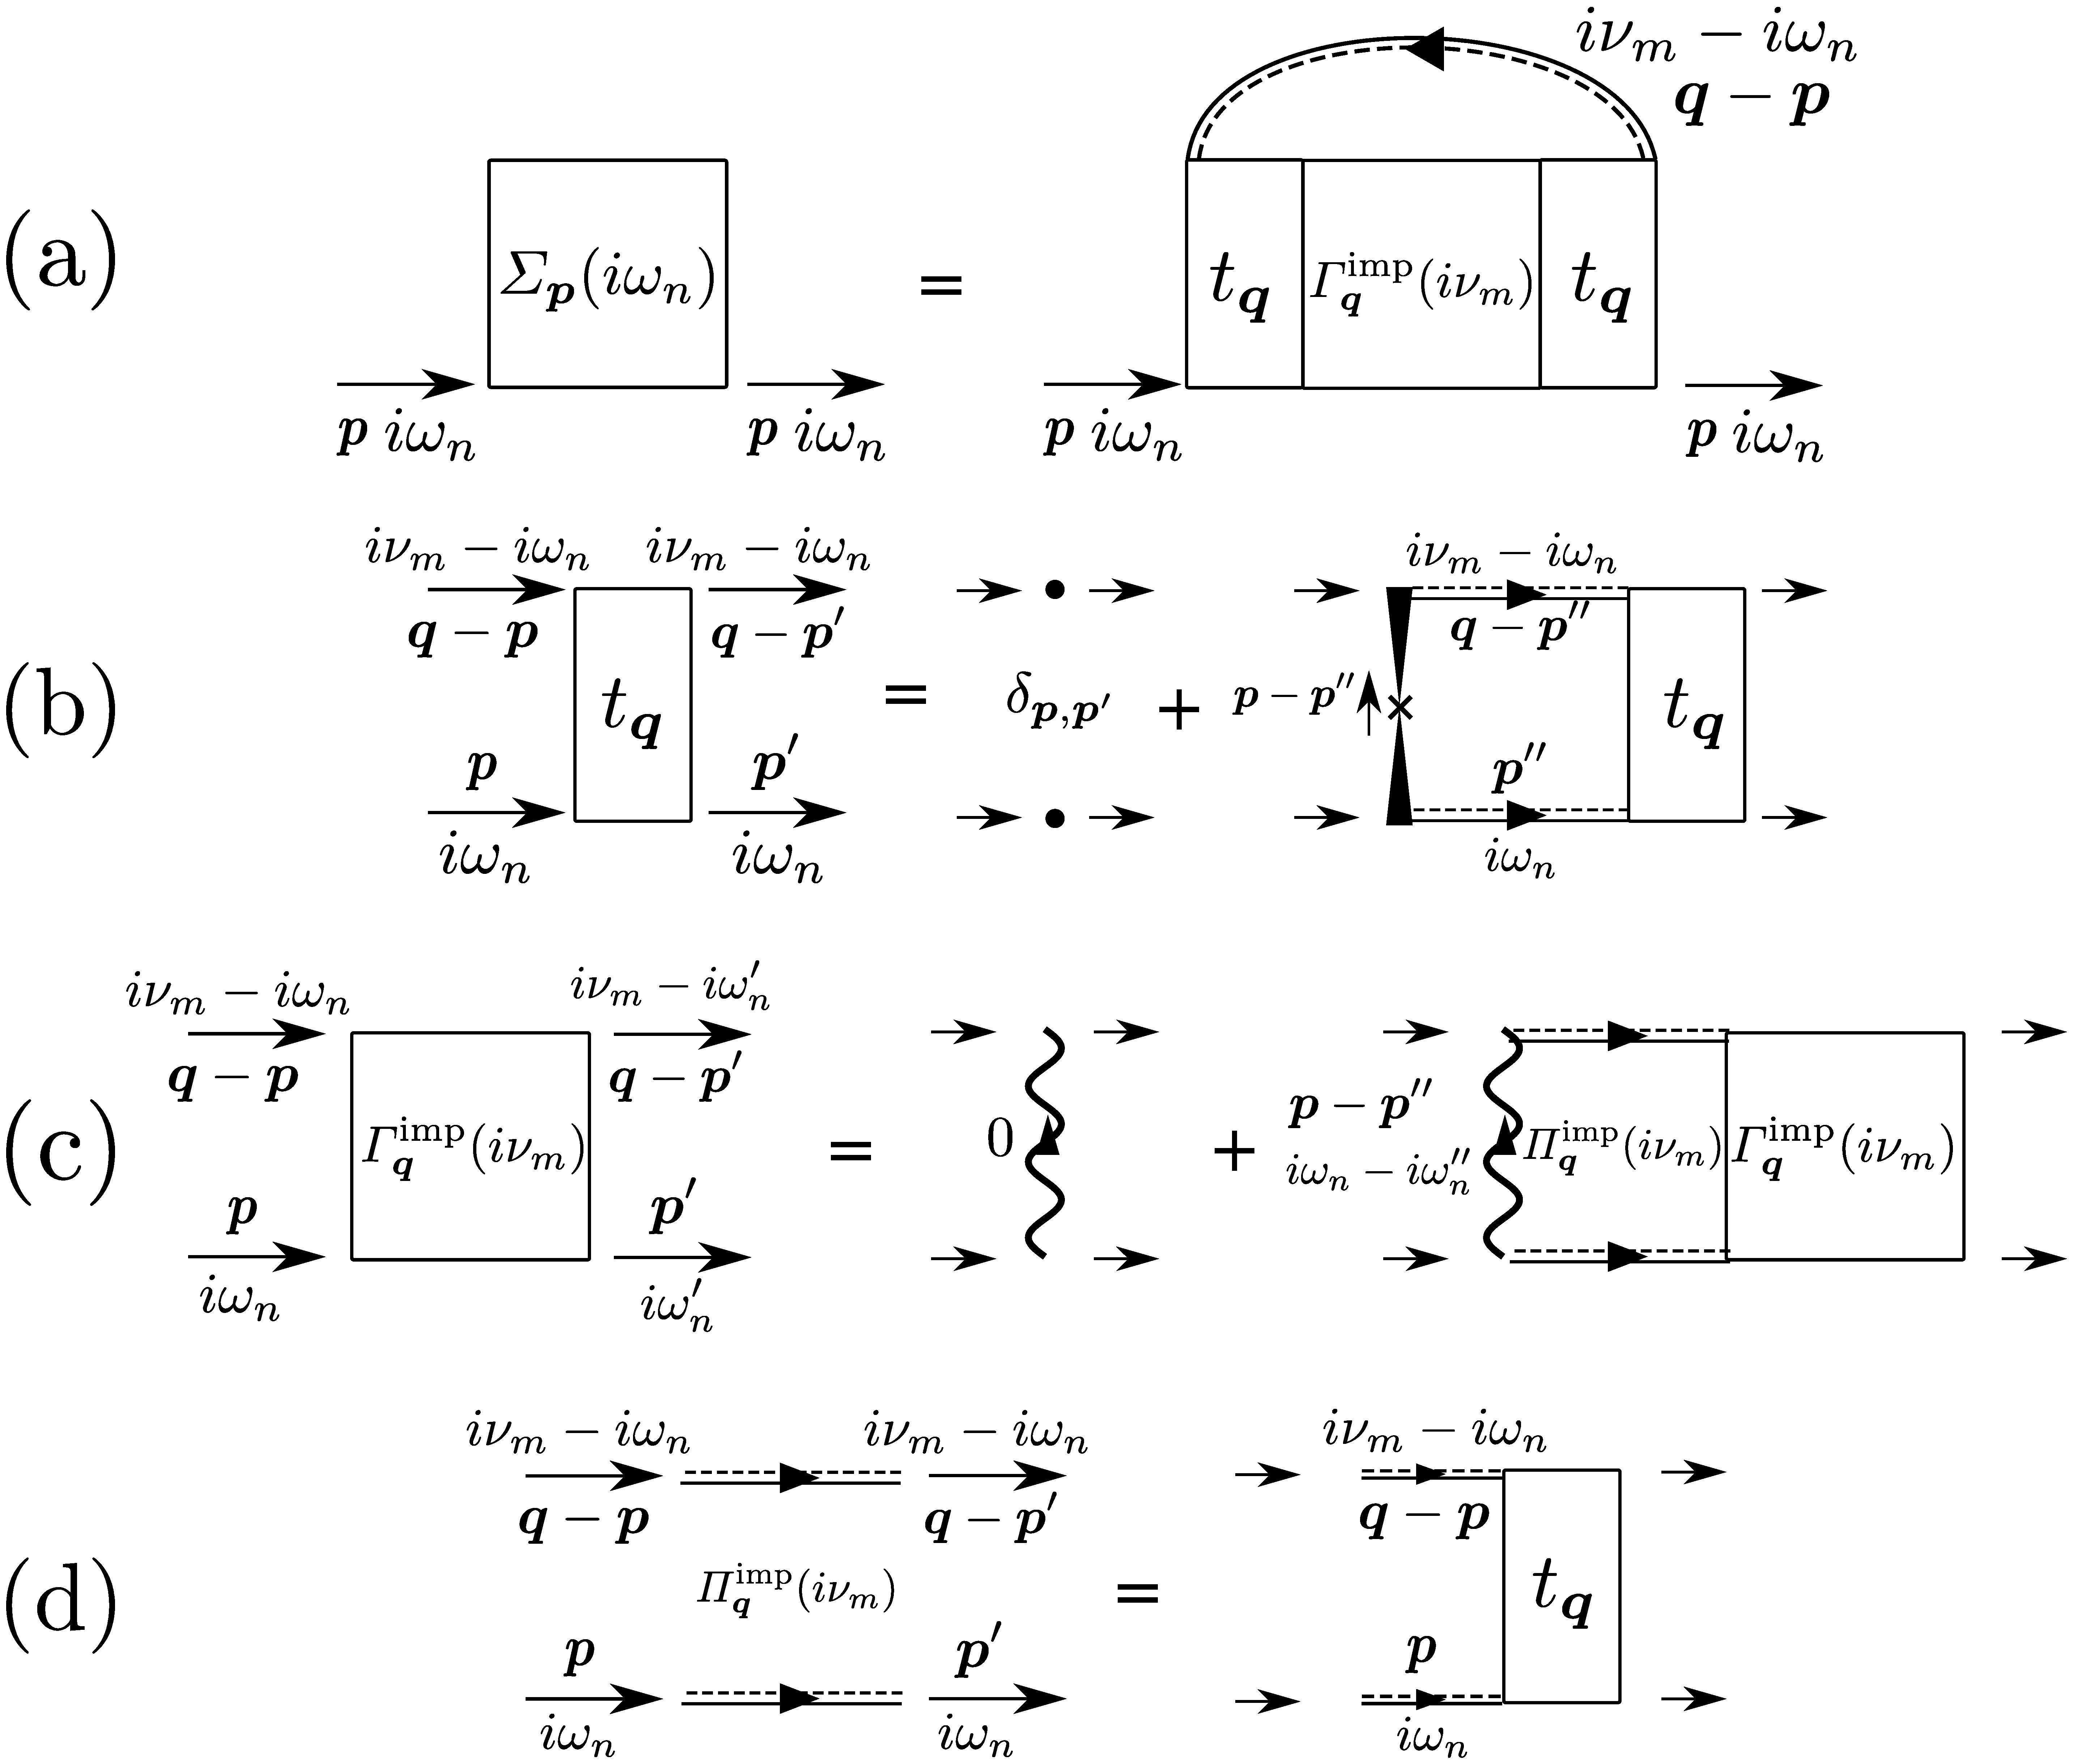
\includegraphics[width=123mm]{eps/sig-gamimpt.eps}
\caption{(a) 非磁性不純物が存在する場合の原子間引力相互作用に対する $T$ 行列近似の自己エネルギー $\sigpom$。破線と実線による二重線は不純物散乱効果の自己エネルギー $\sigimppom$ のみ含むグリーン関数 $\gimppom$、(b) $\vtxp$ は不純物散乱によるバーテックス補正。$\times$ 印は不純物濃度 $c$、黒三角形は図 \ref{fig:form:ham:sigimp} の有効不純物散乱ポテンシャル $\vvtxn$。(c) 引力相互作用に対する $T$ 行列部分 $\gamimpqnu$。 波線は引力相互作用 $-U$。$\piimpqnu$ は引力相互作用に対しては最低次の対相関関数で (d) で与えられる(ただし、上下の $\gimppom$ 線間の不純物散乱は含む)。}
\label{fig:form:tma:sigall}
\label{fig:form:tma:sigvtx}
\label{fig:form:tma:gamimp}
\label{fig:form:tma:piimp}
\end{figure}


BCS-Leggett 理論は、熱揺らぎの効果が影響しない絶対零度においては BCS-BEC クロスオーバー全域で適用可能であるが、有限温度に対しては強結合 BEC 領域を正しく記述できないことが知られている \cite{ohashi2005}。本研究では、ユニタリ極限 $\left(\askfi=0\right)$ における、超流動転移温度 $\tc$ も議論するので、ここでは有限温度の BCS-BEC クロスオーバー現象を扱うことができる $T$ 行列理論を不純物が存在する場合に拡張する。尚、ここでの $T$ 行列理論は原子間引力相互作用に対するものである。不純物散乱効果に対しては前節の $T=0$ の時同様、自己無撞着 $T$ 行列近似のレベルで扱う。本節では超流動転移温度以上の常流動相を扱うため、Nambu 表示ではなく通常の 1 成分表示を用いる。

先ず原子間相互作用に対する無摂動グリーン関数 $\gimppom$ を用意する。ただし、このグリーン関数は非磁性不純物散乱効果は自己無撞着 $T$ 行列近似の範囲で考慮されているとする。すると $\gimppom$ は次式で与えられる。
\beq
\gimppom &= \frac{1}{i \omn - \left[ \ken_{\bp}-\cpt\right] - \sigimppom}\notag\\
&\equiv \frac{1}{i \tomn - \left[ \ken_{\bp}-\tcptn\right]},\label{eq:form:tma:gimp}
\eeq
ここで不純物散乱効果を表す自己エネルギー部分 $\sigimppom$ は式 (\ref{eq:form:ham:sctma}) で与えられる。式 (\ref{eq:form:tma:gimp}) を引力相互作用の摂動展開における無摂動のグリーン関数として用い、図 \ref{fig:form:tma:greenall} で与えられるダイソン方程式を考える。図 \ref{fig:form:tma:greenall} を式で表すと、
\beq
\left[\gpom\right]^{-1} = \left[ \gimppom\right]^{-1} - \sigpom.\label{eq:form:tma:gall}
\eeq
自己エネルギー部分 $\sigpom$ は、原子間引力相互作用 $-U$ の効果を表し、(相互作用に対する)$T$ 行列近似の枠組みでは図 \ref{fig:form:tma:sigall} (a) のダイアグラムで与えられる。これを評価すると、
\beq
&\sigpom = \frac{1}{\beta} \sum_{\nu_m} \sum_{\bq} \gamimpqnu \gimpqnu \left[ \vtxp \right]^2.\label{eq:form:tma:sigpom}
 \eeq
ここで、右辺の $\vtxp$ は図 \ref{fig:form:tma:sigvtx} (b) で与えられ、その表式は次のようになる。
\beq
&\vtxp = \frac{1}{1-c \vvtxn \vvtxmn \pqnmp }.\label{eq:form:tma:vtxp}
\eeq
式 (\ref{eq:form:tma:vtxp}) において、 $\vvtxn$ は式 (\ref{eq:form:ham:sctma}) の有効不純物散乱ポテンシャル、また、$\pqnmp$ は、図 \ref{fig:form:tma:piimp} (d) で上下の $\gimppom$ 線間の不純物散乱を含まない対相関関数であり、
\beq
&\pqnmp = \sum_{\bp} \gimppom \gimpqnu,\label{eq:form:tma:pqnmp}
\eeq
で与えられる。式 (\ref{eq:form:tma:sigpom}) 中の $\gamimpqnu$ は相互作用 $-U$ に対する梯子近似で計算された散乱行列であり、図 \ref{fig:form:tma:gamimp} (c)で与えられる。表式は、
\beq
&\gamimpqnu  =  \frac{-U}{1-U\piimpqnu}.\label{eq:form:tma:gamimp}
\eeq
式 (\ref{eq:form:tma:gamimp}) の $\piimpqnu$ は、対相関関数であり、図 \ref{fig:form:tma:piimp} (d) のダイアグラムから、
\beq
&\piimpqnu =   \frac{1}{\beta} \sumn \pqnmp \vtxp,\label{eq:form:tma:piimp}
\eeq
と与えらえる。



従来の(不純物がない場合の)$T$ 行列を不純物散乱がある場合に拡張することで新たに生じたものが、式 (\ref{eq:form:tma:vtxp}) の 4 点バーテックス $\vtxp$ と、式 (\ref{eq:form:tma:piimp}) の対相関関数 $\piimpqnu$ である。このうち、 $\vtxp$ は、逆向きの擬スピンを有する 2 つのフェルミ原子が同じ不純物に多重散乱され運動量をやり取りする過程を表す。この補正は、無摂動グリーン関数 $\gimppom$ を求める際、不純物散乱に対して自己無撞着 $T$ 行列近似を用いていたことに対応し、式 (\ref{eq:form:ham:sctma}) の有効不純物散乱ポテンシャル $\vvtxn$ による多重散乱の形になっている。一方、対相関関数 $\piimpqnu$ は、金属超伝導の分野でのディフューゾンと呼ばれているものであり、不純物散乱を受けながら伝播する 2 つのフェルミ原子を表す。これを構成単位とし、さらに原子間引力相互作用による散乱を多数回受けた効果を表したものが式 (\ref{eq:form:tma:gamimp}) で与えられる $\gamimpqnu$ である。以上より、式 (\ref{eq:form:tma:gamimp}) を含む自己エネルギー (\ref{eq:form:tma:sigpom}) は、有限温度における超流動揺らぎと、その超流動揺らぎへの非磁性不純物効果を共に含んでいることがわかる。


上述の定式化は、不純物がない場合($c=0$)、従来の BCS-BEC クロスオーバーに対する $T$ 行列近似に帰着する。不純物がない場合の $T$ 行列近似については付録 \ref{sec:append:pure:tma} にまとめた。また、式 (\ref{eq:form:tma:sigpom}) が、前節における絶対零度の BCS-Leggett 理論とコンシステントな理論になっていることは、付録 \ref{sec:append:imptmasf} において説明する。本論文では、$T>0$ の超流動相は扱わないが、付録 \ref{sec:append:imptmasf} では、BCS-Leggett 理論で記述される状態から出発し、超流動ゆらぎに対する対相関関数の応答を線形応答の範囲で計算することで、超流動転移温度 $\tc$ 以下の不純物が存在する場合の $T$ 行列理論を構築する方法についても説明している。尚、この節は常流動相に対する定式化であるが、以下で述べるサウレス条件を用いることで超流動転移温度を決定することは可能である。

こうして求まった $T$ 行列近似を用いる場合、超流動転移温度 $\tc$ はサウレス条件から決定することができる。これは式 (\ref{eq:form:tma:gamimp}) で与えられる散乱行列 $\gamimpqnu$ が低エネルギー、長波長極限で極をもつ条件として超流動転移を与えるものであり、具体的に書き下すと、
\beq
0&=\left[\gamimp_{\bq=0}(i\num=0)\right]^{-1}\notag\\
&=- \frac{1}{U} + \piimp_{\bq=0}(i\num=0)\notag\\
&= \frac{m}{4 \pi \as} +\sum_{\bm{p}} \left[\frac{1}{\beta} \sumn\left[\gimppom \gimp_{-\bp}(-i\omn) t_{\bq=\bm{0}}(i\omn, -i\omn)\right] - \frac{1}{2 \ken_{\bp}}\right],\label{eq:form:tma:th0000}
\eeq
となる。ここで、
\beq
t_{\bq=\bm{0}}(i\omn, -i \omn)& = \frac{1}{1-c \vvtxn \vvtx(-i\omn) \sum_{\bp}\gimppom \gimp_{-\bp}(-i\omn)}\notag\\
&= \frac{1}{1+ \frac{1}{\tomn} \im \sigimppom } \notag\\
&= \frac{\tomn}{\omn},
\eeq
のように、不純物バーテックス補正 $t_{\bq=\bm{0}}(i\omn, -i \omn)$ が、不純物のくりこみを受けた松原周波数と裸の松原周波数の比に一致することを用いれば、式 (\ref{eq:form:tma:th0000}) は、
\beq
0 = \frac{m}{4 \pi \as} +\sum_{\bm{p}}\left[ \left[\frac{1}{\beta} \sumn \frac{\tomn}{\omn} \frac{1}{\tomn^2 + (\ken_p-\tcpt)^2} \right]- \frac{1}{2 \ken_p}\right],\label{eq:form:tma:thouless}
\eeq
となる。式 (\ref{eq:form:tma:thouless}) は、式 (\ref{eq:form:mnf:gapeq}) の BCS-Leggett 理論のギャップ方程式において 式 (\ref{eq:form:mnf:nonmag}) を用いた上で、$\varDelta = 0$ として求めた超流動転移温度を決定する方程式と一致している。

$T$ 行列近似の枠組みで $T_c$ を決定する際に必要なもう 1 つの方程式は、粒子数方程式である。これは通常の手順に従い 1 粒子グリーン関数から次のように得られる。
\beq
N = \sum_{\bp, \spin} \braket{c^{\dag}_{\bp,\spin}c_{\bp,\spin}} = \frac{2}{\beta}\sum_{\bp}\sumn \gpom e^{i \omn \delta}.\label{eq:form:tma:number}
\eeq
今の場合、$\gpom$ は式 (\ref{eq:form:tma:gall}) で与えられる。


以上より、非磁性不純物を含む $T$ 行列近似の枠組みにおいて、$\tc$ は次のように計算される。先ず、式 (\ref{eq:form:tma:gimp}) と 式 (\ref{eq:form:ham:sctma}) から $\gimppom$ を求め、その $\gimppom$ を用いて、式 (\ref{eq:form:tma:gall}) から式 (\ref{eq:form:tma:piimp}) によってグリーン関数 $\gpom$ を計算する。$\gpom$ から、粒子数方程式 (\ref{eq:form:tma:number}) を計算し、サウレスの判定条件 (\ref{eq:form:tma:thouless}) と自己無撞着に解くことによって、超流動転移温度 $\tc$ とその時の化学ポテンシャル $\cpt(T=\tc)$ を決定する。本論文では以上の計算を数値的に行う。


